\documentclass{article}
\usepackage[zh]{homework}
\usepackage{tikz}
\usepackage{placeins}

\config{Algebra-1}{2026 秋季}{1}

\begin{document}

\textbf{我承诺, 本次作业的完成没有使用大语言模型. }

\begin{problem}
  {\heiti 恒等态射与逆态射}(\textbf{identity and inverse morphisms}). 设 $\mathcal C$ 是一个范畴.

  \begin{enumerate}
    \item[(a)] 设
      \[
        f:X\to Y,\qquad r,s:Y\to X
      \]
      满足
      \[
        r\circ f=\id_X,\qquad f\circ s=\id_Y.
      \]
      此时分别称 $r$ 为 $f$ 的左逆(left inverse), $s$ 为 $f$ 的右逆(right inverse). 证明 $r=s$, 并由此证明逆态射的唯一性. 进一步, 若 $X\xrightarrow{f}Y\xrightarrow{g}Z$ 均为同构(isomorphisms), 证明
      \[
        (g\circ f)^{-1}=f^{-1}\circ g^{-1}.
      \]

    \item[(b)] 在集合范畴(category of sets) $\mathbf{Set}$ 中, 令
      \[
        i:\{0\}\longrightarrow\{0,1\},\qquad i(0)=0,
      \]
      并令 $r:\{0,1\}\to\{0\}$ 为唯一的映射. 计算 $r\circ i$ 和 $i\circ r$, 说明为什么``有左逆''和``有右逆''都不能单独作为同构的定义.
  \end{enumerate}
\end{problem}

\begin{solution}
	(a) 根据恒等态射的定义以及结合律,
	\[ r = r \circ \id_Y = r \circ (f \circ s)
	= (r \circ f) \circ s = \id_X \circ s = s. \]
	因此, 如果 $f\in \Hom_{\mathcal{C}}(X,Y)$ 有两个逆, 记为 $g_1, g_2 \in \Hom_{\mathcal{C}}(Y,X)$, 则有 $f \circ g_1 = \id_Y$, 并且 $g_2 \circ f = \id_X$, 因此 $g_1=g_2$.

	下面来证明 $(g\circ f)^{-1} = f^{-1}\circ g^{-1}$. 直接的计算给出
	\begin{align*}
		(g\circ f) \circ (f^{-1}\circ g^{-1})
		&= g \circ (f\circ f^{-1}) \circ g^{-1} 
		= g\circ \id_Y \circ g^{-1}
		= g\circ g^{-1} = \id_Z,\\
		(f^{-1}\circ g^{-1}) \circ (g\circ f) 
		&= f^{-1} \circ (g^{-1} \circ g) \circ f
		= f^{-1} \circ \id_Y \circ f
		= f^{-1} \circ f = \id_X.
	\end{align*}

	(b) 计算表明: $(r \circ i) (0) = 0$, 而
	\[ (i \circ r) (0) = (i \circ r) (1) = 0. \]
	此时, $i$ 的左逆为 $r$, $r$ 的右逆为 $i$, 但是 $i$ 和 $r$ 均不是对方的逆态射.
\end{solution}



\begin{problem}
  {\heiti 由关系构造范畴}(\textbf{categories associated with relations}). 设 $S$ 是集合, $R\subseteq S\times S$ 是一个关系(relation). 考虑以下候选范畴 $\mathcal C_R$: 对象为 $S$ 的元素, 并规定
  \[
    \Hom_{\mathcal C_R}(x,y)=
    \begin{cases}
      \{u_{x,y}\}, & xRy,\\
      \varnothing, & \text{其他情况}.
    \end{cases}
  \]
  复合预定为 $u_{y,z}\circ u_{x,y}=u_{x,z}$.

  \begin{enumerate}
    \item[(a)] 证明: 上述数据能够定义一个范畴, 当且仅当 $R$ 满足自反性(reflexivity)和传递性(transitivity). 写出恒等态射, 并验证结合律(associativity).

    \item[(b)] 假设上述数据定义了范畴. 证明
      \[
        x\cong y\qquad\Longleftrightarrow\qquad xRy\mathbin{\text{ 且 }}yRx,
      \]
      其中 $x\cong y$ 表示对象 $x$ 与 $y$ 之间存在同构. 进一步证明, $\mathcal C_R$ 是群胚, 当且仅当 $R$ 还满足对称性(symmetry). 因此, 等价关系(equivalence relation)给出群胚, 而偏序(partial order)给出的范畴中两个对象同构当且仅当它们相等.

    \item[(c)] 分别计算下列范畴的态射总数、对象的同构类, 以及每个对象的自同构群(automorphism group):
      \begin{enumerate}
        \item[(i)] $S=\{1,2,3,6\}$, 关系为整除(divisibility);
        \item[(ii)] $S=\{0,1,2,3\}$, 关系为``具有相同的奇偶性''.
      \end{enumerate}
  \end{enumerate}
\end{problem}

\begin{solution}
	(a) 先来证明: 如果 $R$ 满足自反性和传递性, 则 $\mathcal{C}_R$ 是范畴. 由于 $xRx$, 因此 $\Hom_{\mathcal{C}_R}(x,x) = \{u_{x,x}\}$, 即恒等态射存在; 由于 $xRy, yRz \implies xRz$, 因此若 $u_{x,y}$ 和 $u_{y,z}$ 存在, 则 $u_{x,z} = u_{y,z} \circ u_{x,y}$ 存在. 并且, 由复合的定义, 结合律和恒等态射的性质天然成立(详细见下文). 因此 $\mathcal{C}_R$ 是范畴.

	再来证明: 若 $\mathcal{C}_R$ 是一个范畴, 则 $R$ 满足自反性和传递性. 由于对于任意一个对象 $x$, 均有 $\id_x \in \Hom_{\mathcal{C}_R}(x,x)$, 因此后者非空, 因此 $xRx$, 自反性成立; 若 $xRy$ 且 $yRz$, 则 $u_{x,z} = u_{y,z} \circ u_{x,y}$ 存在, 即 $xRz$, 因此传递性成立.

	对于每一个对象 $x$, 其恒等态射即为 $u_{x,x}$. 对于满足 $xRy$, $yRz$, $zRw$ 的对象 $x,y,z,w$, 有
	\begin{align*}
		u_{z,w} \circ (u_{y,z} \circ u_{x,y})
		&= u_{z,w} \circ u_{x,z}
		= u_{x,w} \\
		&= u_{y,w} \circ u_{x,y}
		=(u_{z,w} \circ u_{y,z}) \circ u_{x,y}.
	\end{align*}
	因此结合律成立.

	(b) 先证明第一个命题. 若 $x,y$ 之间存在同构, 则 $\Hom_{\mathcal{C}_R}(x,y)$ 与 $\Hom_{\mathcal{C}_R}(y,x)$ 均非空, 即 $xRy$ 且 $yRx$; 反过来, 若 $xRy$ 且 $yRx$, 则 $u_{x,y}$ 与 $u_{y,x}$ 均存在. 而根据结合律, 	\[ u_{y,x} \circ u_{x,y} = u_{x,x} = \id_x,\quad 
	u_{x,y} \circ u_{y,x} = u_{y,y} = \id_y, \]
	因此 $u_{x,y} = u_{y,x}^{-1}$, 从而两者皆为同构, 因此 $x \cong y$.

	再证明第二个命题. 若 $\mathcal{C}_R$ 是群胚, 则每一个态射都是同构, 因此都有逆态射. 因此, 若 $xRy$, 则 $u_{x,y}$ 存在, 因此 $u_{y,x}$ 存在, 从而 $yRx$. 这说明 $R$ 具有对称性; 反过来, 若 $R$ 具有对称性, 则对于满足 $xRy$ 的对象 $x,y$, 由 $yRx$ 知 $u_{y,x}$ 存在, 即 $u_{x,y}$ 存在逆态射, 所以为同构. 因此 $\mathcal{C}_R$ 为群胚.

	(c) 这两个范畴的示意图如图 \ref{category_sketch} 所示. 第一个范畴拥有 $9$ 个态射, 每个对象单独为一个同构类; 第二个范畴拥有 $8$ 个态射, 同构类为 $\{0,2\}$ 和 $\{1,3\}$. 所有的对象的自同构群均为平凡群 $\{e\}$.
	\begin{figure}[htbp]
		\centering
		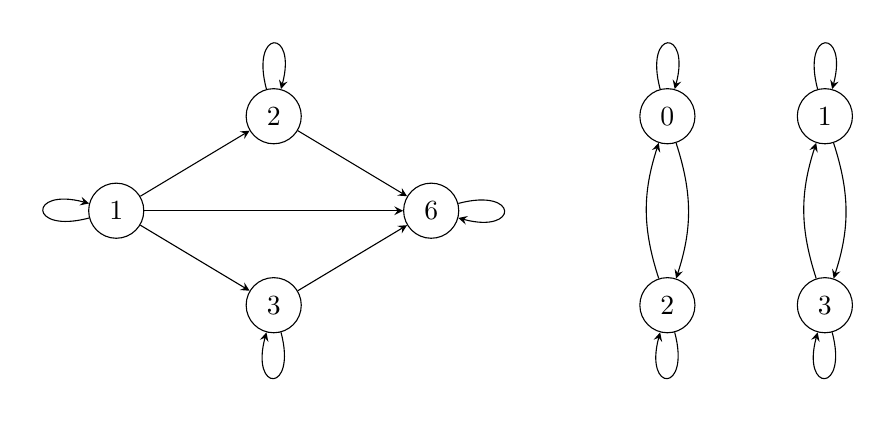
\begin{tikzpicture}[
			>=stealth,
			vertex/.style={circle, draw, minimum size=7mm, inner sep=0pt},
			every loop/.style={min distance=8mm, looseness=6}
		]
			% 整除关系对应的范畴
			\node[vertex] (d1) at (0,0) {$1$};
			\node[vertex] (d2) at (2,1.2) {$2$};
			\node[vertex] (d3) at (2,-1.2) {$3$};
			\node[vertex] (d6) at (4,0) {$6$};
			\path[->]
				(d1) edge[loop left] (d1)
				(d2) edge[loop above] (d2)
				(d3) edge[loop below] (d3)
				(d6) edge[loop right] (d6)
				(d1) edge (d2)
				(d1) edge (d3)
				(d1) edge (d6)
				(d2) edge (d6)
				(d3) edge (d6);

			% 相同奇偶性关系对应的范畴
			\node[vertex] (p0) at (7,1.2) {$0$};
			\node[vertex] (p2) at (7,-1.2) {$2$};
			\node[vertex] (p1) at (9,1.2) {$1$};
			\node[vertex] (p3) at (9,-1.2) {$3$};
			\path[->]
				(p0) edge[loop above] (p0)
				(p2) edge[loop below] (p2)
				(p1) edge[loop above] (p1)
				(p3) edge[loop below] (p3)
				(p0) edge[bend left=18] (p2)
				(p2) edge[bend left=18] (p0)
				(p1) edge[bend left=18] (p3)
				(p3) edge[bend left=18] (p1);
		\end{tikzpicture}
		\caption{两个范畴的示意图}
		\label{category_sketch}
	\end{figure}
	\FloatBarrier
\end{solution}



\begin{problem}
  {\heiti 相反范畴}(\textbf{opposite category}){\heiti 与群胚核心}(\textbf{groupoid core}).

  \begin{enumerate}
    \item[(a)] 对范畴 $\mathcal C$, 定义 $\mathcal C^{\mathrm{op}}$ 的对象与 $\mathcal C$ 相同, 并令
      \[
        \Hom_{\mathcal C^{\mathrm{op}}}(X,Y)=\Hom_{\mathcal C}(Y,X).
      \]
      将 $f:X\to Y$ 对应的态射记为 $f^{\mathrm{op}}:Y\to X$. 对于 $\mathcal C$ 中的 $X\xrightarrow{f}Y\xrightarrow{g}Z$, 规定
      \[
        f^{\mathrm{op}}\circ g^{\mathrm{op}}=(g\circ f)^{\mathrm{op}},\qquad
        \id^{\mathcal C^{\mathrm{op}}}_X=(\id^{\mathcal C}_X)^{\mathrm{op}}.
      \]
      验证这些数据定义一个范畴, 并写出
      \[
        (\mathcal C^{\mathrm{op}})^{\mathrm{op}}\cong\mathcal C
      \]
      在对象和态射上的对应. 解释为什么 $f^{\mathrm{op}}$ 与 $f^{-1}$ 不是同一个概念.

    \item[(b)] 定义 $\mathcal C^{\simeq}$ 的对象与 $\mathcal C$ 相同, 并令
      \[
        \Hom_{\mathcal C^{\simeq}}(X,Y)=\operatorname{Isom}_{\mathcal C}(X,Y),
      \]
      其中右端是从 $X$ 到 $Y$ 的所有同构组成的集合; 复合与恒等态射继承自 $\mathcal C$. 验证 $\mathcal C^{\simeq}$ 是群胚. 进一步证明, 对任意对象 $X$, $\operatorname{Aut}_{\mathcal C}(X)$ 在复合运算下是一个群(group); 这里不需要假设 $\mathcal C$ 本身是群胚.
  \end{enumerate}
\end{problem}

\begin{problem}
  {\heiti 切片范畴、余切片范畴与对偶}(\textbf{duality}). 固定范畴 $\mathcal C$ 中的对象 $A$.

  定义切片范畴(slice category, 又称 overcategory) $\mathcal C/A$: 对象是态射 $p:X\to A$; 从 $p:X\to A$ 到 $q:Y\to A$ 的态射是满足 $q\circ u=p$ 的态射 $u:X\to Y$.

  定义余切片范畴(coslice category, 又称 undercategory) $A/\mathcal C$: 对象是态射 $p:A\to X$; 从 $p:A\to X$ 到 $q:A\to Y$ 的态射是满足 $u\circ p=q$ 的态射 $u:X\to Y$.

  \begin{enumerate}
    \item[(a)] 在上述两个构造中, 分别定义恒等态射与复合, 验证复合仍然满足所要求的交换条件(commutativity condition), 并验证范畴公理.

    \item[(b)] 在 $\mathbf{Set}/A$ 中, 取
      \[
        A=\{0,1\},\qquad X=\{1,2,3\},\qquad Y=\{u,v,w\},
      \]
      并定义
      \[
        p(1)=p(2)=0,\quad p(3)=1,\qquad q(u)=0,\quad q(v)=q(w)=1.
      \]
      列出 $\Hom_{\mathbf{Set}/A}(p,q)$ 中的全部态射. 对象 $p$ 与 $q$ 是否同构? 比较这个问题与``集合 $X$ 和 $Y$ 是否同构''.

    \item[(c)] (选做)尝试想象有如下结果, 如何理解和严谨的定义和说明:
      \[
        (\mathcal C/A)^{\mathrm{op}}\cong A/\mathcal C^{\mathrm{op}},\qquad
        (A/\mathcal C)^{\mathrm{op}}\cong\mathcal C^{\mathrm{op}}/A.
      \]
  \end{enumerate}
\end{problem}

\begin{problem}
  {\heiti 反变函子}(\textbf{contravariant functor}){\heiti 的定义与集合上的例子}. 定义. 从范畴 $\mathcal C$ 到范畴 $\mathcal D$ 的一个反变函子 $F$ 由以下数据组成: 对每个对象 $X\in\operatorname{Ob}(\mathcal C)$, 指定对象 $F(X)\in\operatorname{Ob}(\mathcal D)$; 对每对对象 $X,Y$, 指定集合映射
  \[
    F_{X,Y}:\Hom_{\mathcal C}(X,Y)\longrightarrow
    \Hom_{\mathcal D}(F(Y),F(X)).
  \]
  将 $F_{X,Y}(f)$ 简记为 $F(f)$. 这些数据必须满足
  \[
    F(\id_X)=\id_{F(X)}
  \]
  以及: 对每一对可复合态射 $X\xrightarrow{f}Y\xrightarrow{g}Z$, 有
  \[
    F(g\circ f)=F(f)\circ F(g)\qquad\text{于 }\Hom_{\mathcal D}(F(Z),F(X)).
  \]

  \begin{enumerate}
    \item[(a)] 证明: 给出上述意义下的反变函子, 等价于给出一个协变函子
      \[
        \widetilde F:\mathcal C^{\mathrm{op}}\longrightarrow\mathcal D,
      \]
      其中 $\widetilde F(X)=F(X)$, $\widetilde F(f^{\mathrm{op}})=F(f)$. 逐项比较两种表述中的恒等态射公理和复合公理.

    \item[(b)] 对集合 $X$, 记其幂集(power set)为 $\mathcal P(X)$. 对映射 $f:X\to Y$, 用逆像(inverse image)定义
      \[
        \mathcal P^*(f^{\mathrm{op}}):\mathcal P(Y)\longrightarrow\mathcal P(X),\qquad
        B\longmapsto f^{-1}(B).
      \]
      证明这定义一个函子 $\mathcal P^*:\mathbf{Set}^{\mathrm{op}}\to\mathbf{Set}$, 即从 $\mathbf{Set}$ 到 $\mathbf{Set}$ 的一个反变函子.

      具体取
      \[
        X=\{1,2,3\},\qquad Y=\{a,b\},\qquad f(1)=f(2)=a,\quad f(3)=b.
      \]
      计算 $\mathcal P^*(f^{\mathrm{op}})$ 在 $\mathcal P(Y)$ 的每个元素上的值.

    \item[(c)] 同样的对象赋值 $X\mapsto\mathcal P(X)$, 配上直接像(direct image)映射
      \[
        \mathcal P_*(f):\mathcal P(X)\longrightarrow\mathcal P(Y),\qquad B\longmapsto f(B),
      \]
      是否定义一个协变函子 $\mathcal P_*:\mathbf{Set}\to\mathbf{Set}$? 验证你的结论.
  \end{enumerate}
\end{problem}

\begin{problem}
  {\heiti 函子的复合}(\textbf{composition of functors}).

  \begin{enumerate}
    \item[(a)] 设 $F:\mathcal C\to\mathcal D$、$G:\mathcal D\to\mathcal E$ 是协变函子. 定义
      \[
        (G\circ F)(X)=G(F(X)),\qquad (G\circ F)(f)=G(F(f)).
      \]
      验证 $G\circ F$ 是一个函子, 且
			\begin{gather*}
	      (G\circ F)(\id_X)=\id_{(G\circ F)(X)}, \\
	      (G\circ F)(g\circ f)=(G\circ F)(g)\circ(G\circ F)(f).
			\end{gather*}

    \item[(b)] 定义恒等函子(identity functor) $\id_{\mathcal C}$, 并在对象与态射两个层面验证
      \[
        F\circ\id_{\mathcal C}=F,\qquad
        \id_{\mathcal D}\circ F=F,
      \]
      以及
      \[
        H\circ(G\circ F)=(H\circ G)\circ F
      \]
      对所有可复合的协变函子成立.

    \item[(c)] (选做)对任意协变函子 $K:\mathcal A\to\mathcal B$, 定义相反函子(opposite functor)
      \[
        K^{\mathrm{op}}:\mathcal A^{\mathrm{op}}\longrightarrow\mathcal B^{\mathrm{op}},\qquad
        K^{\mathrm{op}}(X)=K(X),\qquad K^{\mathrm{op}}(u^{\mathrm{op}})=K(u)^{\mathrm{op}}.
      \]
      验证 $K^{\mathrm{op}}$ 是函子.

      利用这一构造, 检查下表中各个复合的定义域(domain)与陪域(codomain), 并验证其函子公理. 将 $(\mathcal C^{\mathrm{op}})^{\mathrm{op}}$ 与 $\mathcal C$ 按第 3 题的对应识别.
      \[
        \begin{array}{c|c|c}
          F & G & \text{合法的复合}\\ \hline
          F:\mathcal C^{\mathrm{op}}\to\mathcal D & G:\mathcal D\to\mathcal E & G\circ F:\mathcal C^{\mathrm{op}}\to\mathcal E\\
          F:\mathcal C\to\mathcal D & G:\mathcal D^{\mathrm{op}}\to\mathcal E & G\circ F^{\mathrm{op}}:\mathcal C^{\mathrm{op}}\to\mathcal E\\
          F:\mathcal C^{\mathrm{op}}\to\mathcal D & G:\mathcal D^{\mathrm{op}}\to\mathcal E & G\circ F^{\mathrm{op}}:\mathcal C\to\mathcal E
        \end{array}
      \]
      相对于原范畴 $\mathcal C$, 分别指出所得作用是协变(covariant)还是反变(contravariant). 特别解释: ``两个反变作用复合得到协变作用''应当如何用普通函子的复合严格表述.
  \end{enumerate}
\end{problem}

\begin{problem}
  {\heiti 单态射}(\textbf{monomorphism}){\heiti 与满态射}(\textbf{epimorphism}){\heiti : 定义和基本性质}. 定义. 设 $f:X\to Y$ 是范畴 $\mathcal C$ 中的一个态射.

  \begin{itemize}
    \item 若对任意对象 $T$ 和任意两个态射 $a,b:T\to X$, 都有
      \[
        f\circ a=f\circ b\qquad\Longrightarrow\qquad a=b,
      \]
      则称 $f$ 为单态射(monomorphism, 简称 mono).

    \item 若对任意对象 $T$ 和任意两个态射 $a,b:Y\to T$, 都有
      \[
        a\circ f=b\circ f\qquad\Longrightarrow\qquad a=b,
      \]
      则称 $f$ 为满态射(epimorphism, 简称 epi).
  \end{itemize}

  证明以下结论:
  \begin{enumerate}
    \item[(a)] 若 $f$ 有左逆, 证明 $f$ 是单态射; 若 $f$ 有右逆, 证明 $f$ 是满态射. 由此证明每个同构都是单态射和满态射.

    \item[(b)] 对可复合的态射 $X\xrightarrow{f}Y\xrightarrow{g}Z$, 证明:
      \begin{enumerate}
        \item[(i)] 若 $f,g$ 都是单态射, 则 $g\circ f$ 是单态射; 若 $f,g$ 都是满态射, 则 $g\circ f$ 是满态射.
        \item[(ii)] 若 $g\circ f$ 是单态射, 则 $f$ 是单态射; 若 $g\circ f$ 是满态射, 则 $g$ 是满态射.
      \end{enumerate}

    \item[(c)] 用上述定义证明单态射与满态射的对偶关系:
      \[
        f\text{ 在 }\mathcal C\text{ 中是单态射}\qquad\Longleftrightarrow\qquad
        f^{\mathrm{op}}\text{ 在 }\mathcal C^{\mathrm{op}}\text{ 中是满态射},
      \]
      \[
        f\text{ 在 }\mathcal C\text{ 中是满态射}\qquad\Longleftrightarrow\qquad
        f^{\mathrm{op}}\text{ 在 }\mathcal C^{\mathrm{op}}\text{ 中是单态射}.
      \]
  \end{enumerate}
\end{problem}

\begin{problem}
  \begin{enumerate}
    \item[(a)] 在 $\mathbf{Set}$ 中证明
      \[
        f\text{ 是单态射}\qquad\Longleftrightarrow\qquad f\text{ 是单射(injection)},
      \]
      \[
        f\text{ 是满态射}\qquad\Longleftrightarrow\qquad f\text{ 是满射(surjection)}.
      \]
      提示: 分别考虑以单点集为定义域、以两点集为陪域的测试映射.

      由此证明: 在 $\mathbf{Set}$ 中, 一个态射同时是单态射和满态射, 当且仅当它是双射(bijection), 也当且仅当它是同构.

    \item[(b)] 令 $\mathcal I$ 是偏序 $0<1$ 对应的范畴, 即除恒等态射外, 只有一个态射 $u:0\to1$. 证明 $u$ 同时是单态射和满态射, 但不是同构.

      进一步证明: 在任意偏序对应的范畴中, 每个态射都是单态射和满态射. 解释为什么这个反例与上一小题的结论不矛盾.
  \end{enumerate}
\end{problem}

\begin{problem}
  \textbf{Hom} {\heiti 函子}(\textbf{Hom functors}). 固定范畴 $\mathcal C$ 中的对象 $A$.

  \begin{enumerate}
    \item[(a)] 严格的给出定义 $\Hom_{\mathcal C}(A,-):\mathcal C\to\mathbf{Set}$, 满足在态射 $f:X\to Y$ 上的作用为
      \[
        \Hom_{\mathcal C}(A,X)\longrightarrow\Hom_{\mathcal C}(A,Y),\qquad
        u\longmapsto f\circ u.
      \]
      严格的给出定义 $\Hom_{\mathcal C}(-,A):\mathcal C^{\mathrm{op}}\to\mathbf{Set}$ 满足在 $f^{\mathrm{op}}:Y\to X$ 上的作用为
      \[
        \Hom_{\mathcal C}(Y,A)\longrightarrow\Hom_{\mathcal C}(X,A),\qquad
        v\longmapsto v\circ f.
      \]
      验证前者是协变函子, 后者给出从 $\mathcal C$ 到 $\mathbf{Set}$ 的反变函子. 这两种作用分别称为后复合(postcomposition)和预复合(precomposition).

    \item[(b)] 给定 $f:X\to Y$, 对每个对象 $T$, 记
      \[
        \begin{aligned}
          f_{*,T}&:\Hom(T,X)\longrightarrow\Hom(T,Y),
          & a&\longmapsto f\circ a,\\
          f_T^*&:\Hom(Y,T)\longrightarrow\Hom(X,T),
          & b&\longmapsto b\circ f.
        \end{aligned}
      \]
      证明
      \[
        \begin{aligned}
          f\text{ 是单态射}&\qquad\Longleftrightarrow\qquad f_{*,T}\text{ 对每个 }T\text{ 都是单射},\\
          f\text{ 是满态射}&\qquad\Longleftrightarrow\qquad f_T^*\text{ 对每个 }T\text{ 都是单射}.
        \end{aligned}
      \]
  \end{enumerate}
\end{problem}

\begin{problem}
  设 $F:\mathcal C\to\mathcal D$ 是函子. 如果对每对对象 $X,Y$, 映射
  \[
    \Hom_{\mathcal C}(X,Y)\longrightarrow
    \Hom_{\mathcal D}(F(X),F(Y))
  \]
  都是单射, 则称 $F$ 为{\heiti 忠实函子}(\textbf{faithful functor}).

  \begin{enumerate}
    \item[(a)] 证明任意函子都保持同构, 并且对同构 $f$ 有
      \[
        F(f^{-1})=F(f)^{-1}.
      \]

    \item[(b)] 证明忠实函子反映单态射和满态射, 即
      \[
        F(f)\text{ 是单态射}\qquad\Longrightarrow\qquad f\text{ 是单态射},
      \]
      \[
        F(f)\text{ 是满态射}\qquad\Longrightarrow\qquad f\text{ 是满态射}.
      \]
  \end{enumerate}
\end{problem}


\end{document}
